\documentclass[tikz,border=8pt]{standalone}

\usepackage{xcolor}
\definecolor{direct}{HTML}{377EB8}

\usepackage{tikz}
\usetikzlibrary{arrows.meta}

\usepackage{lmodern}
\SetSymbolFont{letters}{bold}{OML}{cmbr}{bx}{it}
\renewcommand{\familydefault}{\sfdefault}
\usepackage{sansmathfonts}

\begin{document}

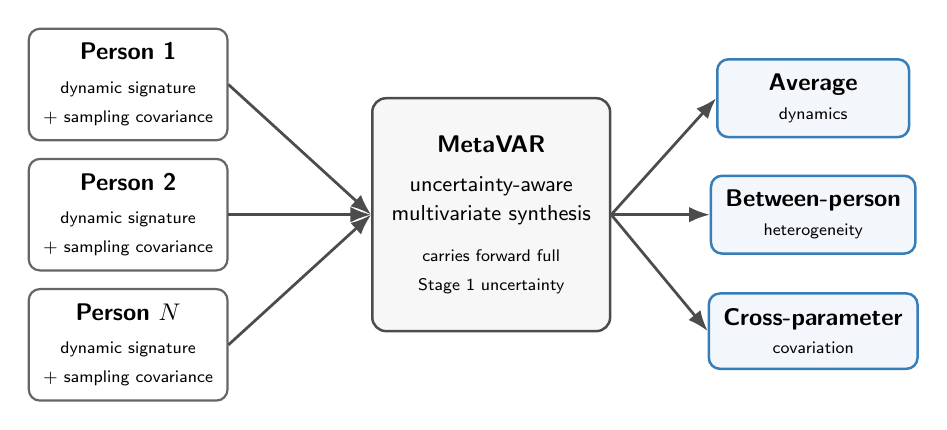
\begin{tikzpicture}[
		x=1cm, y=1cm,
		scale=0.87,
		transform shape,
		>=Latex,
		box/.style={
			draw=black!60,
			rounded corners=4pt,
			line width=0.8pt,
			fill=white,
			align=center,
			inner sep=6pt
		},
		stage/.style={
			draw=black!70,
			rounded corners=5pt,
			line width=0.9pt,
			fill=black!3,
			align=center,
			inner sep=8pt
		},
		outbox/.style={
			draw=direct,
			rounded corners=4pt,
			line width=0.9pt,
			fill=direct!6,
			align=center,
			inner sep=6pt
		},
		arrow/.style={
			->,
			line width=1.0pt,
			draw=black!70
		}
	]
	
	% Person-specific boxes
	\node[box, minimum width=2.6cm, minimum height=1.6cm] (p1) at (1.8,4.2) {%
		\textbf{Person 1}\\[0.2em]
		{\scriptsize dynamic signature}\\
		{\scriptsize $+$ sampling covariance}
	};
	
	\node[box, minimum width=2.6cm, minimum height=1.6cm] (p2) at (1.8,2.3) {%
		\textbf{Person 2}\\[0.2em]
		{\scriptsize dynamic signature}\\
		{\scriptsize $+$ sampling covariance}
	};
	
	\node[box, minimum width=2.6cm, minimum height=1.6cm] (pn) at (1.8,0.4) {%
		\textbf{Person $N$}\\[0.2em]
		{\scriptsize dynamic signature}\\
		{\scriptsize $+$ sampling covariance}
	};
	
	% Central synthesis box
	\node[stage, minimum width=3.1cm, minimum height=3.4cm] (meta) at (7.1,2.3) {%
		\textbf{MetaVAR}\\[0.4em]
		{\small uncertainty-aware}\\
		{\small multivariate synthesis}\\[0.5em]
		{\scriptsize carries forward full}\\
		{\scriptsize Stage 1 uncertainty}
	};
	
	% Output boxes
	\node[outbox, minimum width=2.8cm, minimum height=1.1cm] (avg) at (11.8,4.0) {%
		\textbf{Average}\\
		{\scriptsize dynamics}
	};
	
	\node[outbox, minimum width=2.8cm, minimum height=1.1cm] (het) at (11.8,2.3) {%
		\textbf{Between-person}\\
		{\scriptsize heterogeneity}
	};
	
	\node[outbox, minimum width=2.8cm, minimum height=1.1cm] (cov) at (11.8,0.6) {%
		\textbf{Cross-parameter}\\
		{\scriptsize covariation}
	};
	
	% Arrows from people to MetaVAR
	\draw[arrow] (p1.east) -- (meta.west);
	\draw[arrow] (p2.east) -- (meta.west);
	\draw[arrow] (pn.east) -- (meta.west);
	
	% Arrows from MetaVAR to outputs
	\draw[arrow] (meta.east) -- (avg.west);
	\draw[arrow] (meta.east) -- (het.west);
	\draw[arrow] (meta.east) -- (cov.west);
	
\end{tikzpicture}

\end{document}